\documentclass[default]{beamer}
\setbeamertemplate{navigation symbols}{}

\usetheme{CambridgeUS}
%\useoutertheme{infolines}
\usecolortheme{beaver}

\usepackage[utf8]{inputenc}					% Выбор языка и кодировки
\usepackage[english, russian]{babel}	% Языки: русский, английский
\usepackage{csquotes}
\usepackage{tikz}
\usetikzlibrary{arrows,shapes,calc}
\usepackage{animate}
\usepackage{fp}
\usepackage{media9}
\usepackage{textpos}
\usepackage{hyperref}

\usepackage[
	language=auto,
	autolang=other,
	backend=biber,
	style=authortitle,
	sorting=ydnt,
	maxbibnames=5
]{biblatex}
\addbibresource{panov_isum.bib}
				
\DeclareSourcemap{
	\maps[datatype=bibtex, overwrite]{
		\map{
			\step[fieldset=langid, fieldvalue=english]
			\step[fieldset=doi, null]
			\step[fieldset=issn, null]
			\step[fieldset=isbn, null]
			\step[fieldset=url, null]
			\step[fieldsource=language, fieldset=langid, origfieldval]
		}
	}
}
\DeclareBibliographyDriver{std}{%
	\usebibmacro{bibindex}%
	\usebibmacro{begentry}%
	\usebibmacro{author/editor+others/translator+others}%
	\setunit{\labelnamepunct}\newblock
	\usebibmacro{title}%
	\newunit\newblock
	\usebibmacro{maintitle+booktitle}
	\newunit\newblock
	\usebibmacro{journal}%
	\newunit\newblock
	\usebibmacro{date}%
	\newunit\newblock
	\usebibmacro{finentry}
}
\DeclareBibliographyAlias{article}{std}
\DeclareBibliographyAlias{book}{std}
\DeclareBibliographyAlias{inproceedings}{std}
\DeclareBibliographyAlias{incollection}{std}

\graphicspath{{../../images/}} 			% Пути к изображениям

\makeatletter
\setbeamertemplate{footline}
{
	\leavevmode%
	\hbox{%
		\begin{beamercolorbox}[wd=.333333\paperwidth,ht=2.25ex,dp=1ex,center]{author
				in head/foot}%
			\usebeamerfont{author in
				head/foot}\insertshortauthor~~\beamer@ifempty{\insertshortinstitute}{}{(\insertshortinstitute)}
		\end{beamercolorbox}%
		\begin{beamercolorbox}[wd=.333333\paperwidth,ht=2.25ex,dp=1ex,center]{title in
				head/foot}%
			\usebeamerfont{title in head/foot}\insertshorttitle
		\end{beamercolorbox}%
		\begin{beamercolorbox}[wd=.333333\paperwidth,ht=2.25ex,dp=1ex,right]{date in
				head/foot}%
			\usebeamerfont{date in head/foot}\insertshortdate{}\hspace*{1em}
			\insertframenumber{}\hspace*{2ex} 
		\end{beamercolorbox}
	}%
	\vskip0pt%
}

\addtobeamertemplate{frametitle}{}{
	\begin{textblock*}{100mm}(\textwidth-35pt,-20pt)
		
\includegraphics[width=1.5cm]{misc/logos/frccsc.png}
	\end{textblock*}
}

\newcommand{\predmatr}[3]{
	\node[ell, rectangle, minimum height = 15, minimum width = 7.5]  at (#1 pt,#2 pt) {}; 
	\node[ellf, rectangle, minimum height = 15, minimum width = 7.5] at (#1+7.5 pt,#2 pt) {};
	\node[minimum height = 15, minimum width = 15] (#3) at (#1+3.3pt,#2 pt) {};
	\draw[ell] (#1+7.5 pt,#2+7.5 pt) -- (#1 +7.5 pt,#2-7.5 pt);
}
\renewcommand*{\bibfont}{\tiny}
\setlength\bibitemsep{-5pt}

\begin{document}
	
	\title[Коалицинные задачи]{Коалиционные и коллаборативные задачи в робототехнике и методы их решения}
	\author[Панов]{Осипов Геннадий Семенович\\д.ф.-м.н., зам. директора\\
		\textbf{Александр Игоревич Панов}\\\textbf{к.ф.-м.н., с.н.с.}}
	\institute[ФИЦ ИУ РАН]{Отдел <<Интеллектуальные динамические системы и когнитивные исследования>>\\Институт системного анализа\\ Федеральный исследовательский центр <<Информатика и управление>>\\Российской академии наук}
	\date[29 мая "--- ИСУМ-2018]{29 мая 2018\\Интеллектуальные системы, управление и мехатроника — 2018} 
	
	\begin{frame}
		\titlepage
		\centering
		\includegraphics[width=100pt]{misc/logos/ras.png} \hspace{10pt}
		
\includegraphics[width=80pt]{misc/logos/frccsc.png} \hspace{10pt}
		
\includegraphics[width=20pt]{misc/logos/hse.png}
	\end{frame}

	\begin{frame}
		\tableofcontents
	\end{frame}

	\section{О докладчиках}

	\begin{frame}
		\frametitle{ФИЦ ИУ РАН}
		\begin{center}
			
\includegraphics[width=0.35\textwidth]{misc/logos/frccsc.png}
		\end{center}
		
		\par\bigskip
		\scriptsize
		Федеральный исследовательский центр <<Информатика и управление>> Российской Академии Наук "--- ведущая организация Российской Федерации, специализирующаяся на научных исследованиях в области компьютерных наук и управления.
		
		\textbf{Структурные подразделения:}
		\begin{itemize}
			\item Институт проблем информатики РАН (большие данные, информационная безопасность).
			\item Вычислительный центр РАН (машинное обучение, математическое моделирование).
			\item Институт системного анализа РАН (искусственный интеллект, системный анализ).
		\end{itemize}
		
		\textbf{Базовые кафедры:}
		\begin{itemize}
			\item ФУПМ МФТИ (<<Системные исследования>> и <<Интеллектуальные системы>>).
			\item ВМК МГУ (<<Информационной безопасности>>).
			\item МГТУ, МИРЭА, МАИ.
		\end{itemize}
	\end{frame}
		
	\begin{frame}
		\frametitle{Отдел <<Искусственный интеллект и принятие решений>>}
		
		\begin{columns}
		\begin{column}{0.7\textwidth}
			\small
			Основные направления исследований:
			\begin{itemize}
				\item Искусственный интеллект.
				\item Информационный поиск и анализ текстов (компьютерная лингвистика, психолингвистика, текстовая аналитика).
				\item Системы принятия решений (мультиможножества).
				\item Медицинские экспертные системы.
				\item Робототехнические системы (управление, обучение, планирование).
				\item Компьютерное когнитивные моделирование (модели когнитивных функций, многоагентные системы).
			\end{itemize}
			
			45 научных сотрудников и инженеров, 4 доктора наук, 16 кандидатов наук.
		\end{column}
		\begin{column}{0.3\textwidth}
			\centering
			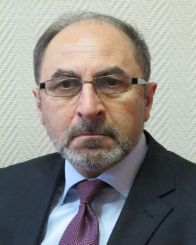
\includegraphics[width=0.4\textwidth]{misc/photos/gs}
			\par\smallskip
			\tiny
			Осипов Геннадий Семенович, зам. дир. ФИЦ ИУ РАН, проф., д.ф.-м.н., президент Российской ассоциации искусственного интеллекта (РААИ)
			\par\medskip
			
\includegraphics[width=0.4\textwidth]{misc/logos/exactus_logo.png}
			\par\medskip
			
\includegraphics[width=0.4\textwidth]{misc/logos/logo_like.png}
			\par\medskip
			
\includegraphics[width=0.4\textwidth]{misc/logos/logo_patent.png}
			
		\end{column}
		\end{columns}
	\end{frame}
		
	\begin{frame}
		\frametitle{Группа управления робототехническими\\системами}
		\footnotesize
		\begin{columns}
		\begin{column}{0.5\textwidth}
		\vspace{-10pt}
		\begin{itemize}
			\item \textbf{Осипов Геннадий Семенович, д.ф.-м.н.},
			\item \textbf{Яковлев Константин Сергеевич, к.ф.-м.н.},
			\item \textbf{Макаров Дмитрий Александрович, к.ф.-м.н.},
			\item \textbf{Панов Александр Игоревич, к.ф.-м.н.},
			\item Даник Юлия, асп. ИСА РАН,
			\item Киселев Глеб, асп. ИСА РАН,
			\item Боковой Андрей, асп. РУДН,
			\item Скрыник Алексей, асп. ИСА РАН,
			\item Ковалев Алексей, асп. ВШЭ,
			\item Андрейчук Антон, асп. ВШЭ,
			\item студенты SLabAI.
		\end{itemize}
		\end{column}
		\begin{column}{0.5\textwidth}
		Основные направления исследований:
		\begin{itemize}
			\item Интеллектуальное управление.
			\item Методы картирования и локализации.
			\item Планирование траекторий.
			\item Машинное обучение.
			\item Моделирование картины мира человека.
			\item Планирование поведения и целеполагание.
			\item Групповое и коалиционное поведение, распределение ролей.
		\end{itemize}
		\end{column}
		\end{columns}		
	\end{frame}	

	\begin{frame}
		\frametitle{Кратко о себе}
		\scriptsize
		\begin{columns}
			\begin{column}{0.85\textwidth}
				\textbf{Панов Александр Игоревич, к. ф.-м. н.}
				\begin{itemize}
					\item Выпускник НГУ и МФТИ.
					\item Старший научный сотрудник отдела <<Интеллектуальные динамические системы и когнитивные исследования>> ФИЦ ИУ РАН.
					\item Научный сотрудник и доцент ФКН ВШЭ.
					\item Доцент кафедры системных исследований Московского физико-технического института (МФТИ).
					\item Член Российской ассоциации искусственного интеллекта (РААИ).
					\item Член Сообщества биологически инспирированных когнитивных архитектур (BICA Society).
					\item Участие в организации международных школ и конференций по биологически инспирированным когнитивным архитектурам (BICA-2016 --- Нью-Йорк, BICA-2017 --- Москва, Fierces on BICA), школы молодых ученых по ИИ (ISyT-2017, Санкт-Петербург), национальной конференции по ИИ (КИИ-2018, RCAI-2018).
					\item Член редколлегии журнала Biologically Inspired Cognitive Architectures.					
					\item Руководитель проектов РФФИ мол\_а, мол\_а\_дк, офи\_м.
					\item Лауреат медали РАН для молодых ученых за 2017 год.
					\item Ментор студенческой лаборатории по ИИ (SLabAI).
				\end{itemize}
			\end{column}
			
			\begin{column}{0.15\textwidth}
				\centering
				\includegraphics[width=\textwidth]{misc/logos/ras.png}
				\vspace{7pt}
				
\includegraphics[width=\textwidth]{misc/logos/frccsc.png}
				\vspace{7pt}
				\includegraphics[width=0.7\textwidth]{misc/logos/isa.png}
				\vspace{7pt}
				\includegraphics[width=0.5\textwidth]{misc/logos/raai.png}
				\vspace{7pt}
				
\includegraphics[width=0.5\textwidth]{misc/logos/hse.png}
				\vspace{7pt}
				\includegraphics[width=\textwidth]{misc/logos/mipt.jpg}
				\vspace{5pt}
				\includegraphics[width=\textwidth]{misc/logos/BICA.png}
				\vspace{5pt}
				\includegraphics[width=0.7\textwidth]{misc/logos/slabai3.png}
			\end{column}
			
		\end{columns}
	\end{frame}

	\section{Коллективное поведение}
	
	\begin{frame}
		\frametitle{Особенности постановки задачи}
		
		Рассматривается случай группового взаимодействия автономных технических объектов (агентов), в котором:
		\begin{itemize}
			\item агенты решают общую задачу (имеют общую цель высшего уровня),
			\item агенты действуют независимо друг от друга (децентрализованное управление), в т.ч. могут ставить индивидуальные подцели и достигать их,
			\item агенты обладают различными характеристиками, как техническими, так и когнитивными, т.е. разными стратегиями поведения,
			\item агенты обладают различными картинами мира,
			\item агенты действуют в меняющейся среде.
		\end{itemize}
		
	\end{frame}
	
	\begin{frame}
		\frametitle{Требования к представлению знаний}
		
		На представление пространственных и временных знаний в задаче согласованного перемещения с такими особенностями налагается ряд ограничений:
		\begin{itemize}
			\item необходимость поддержки некоторого протокола коммуникации, разделение знаний на коммуницируемые и некоммуницируемые (личные),
			\item необходимость выделения компоненты знания, не зависящей от индивидуальных (личных) характеристик агента,
			\item требование к наличию механизма связывания реальных объектов внешней среды и процедур их распознавания с символьным коммуницируемым представлением (symbol grounding problem),
			\item поддержка механизмов пополнения знаний о среде, о себе и о других участниках коалиции (обучение и абстрагирование).
		\end{itemize}
	\end{frame}
	
	\begin{frame}
		\frametitle{Практические задачи}
		
		\centering
		\includegraphics[width=\textwidth]{examples/signs/robotic_signs}
	
	\end{frame}
	
	\begin{frame}
		\frametitle{Задача интеллектуального перемещения}
		
		\begin{columns}
			\begin{column}{0.55\textwidth}
				\begin{center}
					\includegraphics[page=1,width=0.8\textwidth]{examples/plan/slides_colored}
				\end{center}
				\vspace{-7pt}
				\small
				\textbf{Задача}
				
				Целевая область не достижима некоторым агентом самостоятельно (с использованием только методов планирования траектории).
				
				\textbf{Решение}
				
				Агенты должны поддерживать коммуникацию и модифицировать свои собственные планы с учетом коалиционных подзадач.
			
			\end{column}
			\begin{column}{0.45\textwidth}
				Особенности:
				\begin{itemize}
					\item Меняющаяся внешняя среда.
					\item Различные типы препятствий (некоторые могут быть разрушены).
					\item Агенты обладают различной функциональностью.
					\item Общая пространственная цель (ВСЕ агенты должны достичь определенной области на карте).
				\end{itemize}
			\end{column}
		\end{columns}
	\end{frame}
	
	\begin{frame}
		\frametitle{Распределение ролей при решении задачи}
		\begin{center}
			\scalebox{0.7}{
			\animategraphics{12}{examples/plan/slides_colored}{}{}			
			}
		\end{center}
	\end{frame}

	\begin{frame}
		\frametitle{Декомпозиция задачи}
		\footnotesize
		
		\begin{columns}
			\begin{column}{0.6\textwidth}
				\textbf{Декомпозиция} исходной задачи управления коалицией на ряд взаимосвязанных подзадач, каждая из которых решается с привлечением своих способов представления информации, методов и алгоритмов.
				\begin{itemize}
					\item Приобретение концептуальных знаний и планирование действий.
					\item Локализация, картирование (построение модели местности) и планирование траектории.
					\item Выработка управляющего сигнала в виде обратной связи, определение геометрических ограничений на траекторию.
				\end{itemize}
				
			\end{column}
			\begin{column}{0.4\textwidth}
				\includegraphics[width=\textwidth]{agent-schemas/ru/architecture}
			\end{column}
	
		\end{columns}
		\vspace{-5pt}
		\nocite{*}
		\printbibliography[keyword={strl}, resetnumbers=true]
	\end{frame}
	
	\begin{frame}
		\frametitle{Архитектура STRL}
		\centering
		\includegraphics[width=0.65\textwidth]{agent-schemas/ru/architecture}
	\end{frame}
			
	\section{Реактивный уровень}
	\begin{frame}
		\frametitle{Реактивный уровень: постановка}
		
		Конструируются регуляторы для слабо нелинейных систем на основе техники SDRE, т.е. предварительно системы представляются в псевдолинейной форме и регуляторы строятся по алгоритму Калмана-Летова
		
		\[\begin{matrix}
		\frac{dx}{dt}=A(x,\varepsilon )x+B(x,\varepsilon )u=({{A}_{0}}+\varepsilon {{A}_{1}}(x))x+({{B}_{0}}+\varepsilon {{B}_{1}}(x))u,\\ x(0)={{x}^{0}} \\ 
		I(u)=\frac{1}{2}\int_{0}^{\infty }{({{x}^{T}}Q(x,\varepsilon )x}+{{u}^{T}}Ru)dt\to \underset{u}{\mathop{\min }}, \\ 
		u(x)=-{{R}^{-1}}{{B}^{T}}(x,\varepsilon )P(x,\varepsilon )x,\\ PA+{{A}^{T}}P-PB{{R}^{-1}}{{B}^{T}}P+Q=0. \\ 
		\end{matrix}\]
		\par\bigskip
		\nocite{*}
		\printbibliography[keyword={control}, resetnumbers=true]
	\end{frame}
	
	\begin{frame}
		\frametitle{Реактивный уровень: задачи}
		
		\begin{columns}
			\begin{column}{0.4\textwidth}
				Стабилизация квадрокоптера
				\par\bigskip
				\par\bigskip
				\par\bigskip
				Задача слежения для квадрокоптера
				\par\bigskip
				\par\bigskip
				\par\bigskip
				Паде-регулятор				
			\end{column}
			\begin{column}{0.6\textwidth}
				\centering
				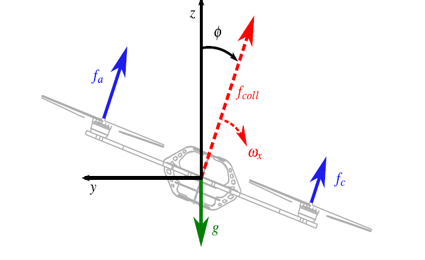
\includegraphics[width=0.48\textwidth]{stabil1.png}
				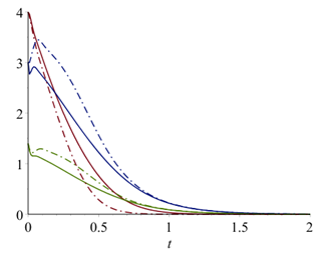
\includegraphics[width=0.48\textwidth]{stabil2.png}
				
				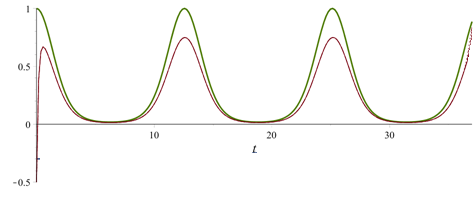
\includegraphics[width=0.8\textwidth]{predict.png}
				
				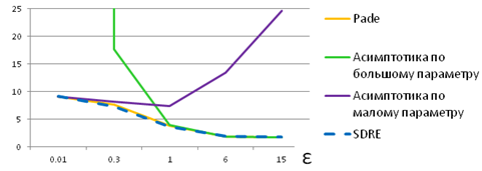
\includegraphics[width=0.9\textwidth]{pade.png}
			\end{column}
		\end{columns}
	\end{frame}
	
	\section{Тактический уровень}
	
	\begin{frame}
		\frametitle{Тактический уровень: планирование траекторий}
		\tiny
		\begin{columns}
			\begin{column}{0.5\textwidth}
				\begin{enumerate}
					\item Агент(ы) моделируется открытым диском радиуса $r$.
					\item Агент(ы) перемещается с учетом кинематических ограничений на возможные направления движения.
					\item Агент(ы) движется с постоянной скоростью $v$, может мгновенно останавливаться и набирать эту скорость (инерционные эффекты не учитываются).
					\item Окружающая среда полностью наблюдаема, cодержит статические препятствия, динамическими препятствиями являются другие агенты и их траектории известны.
					\item Рабочая область (workspace) $U$ - прямоугольник, состоящий из \textit{Free Space} (проходимого пространства) и \textit{Obstacles} (статических препятствий).
					\item Состояние – точка на плоскости: $pos=(x, y)$, начальное и целевое состояние, $s$ и $g$, фиксированы.
					\item Задана функция $los: U \times U \rightarrow \{true, false\}$, определяющая допустимость перехода агента из одного состояния в другое. $los(pos_i, pos_j) = true\ iif\ seg(pos_i, pos_j) \cap Obstacles = \varnothing$, где $seg(pos_1, pos_2)$ - отрезок прямой соединяющий $pos_1$ и $pos_2$.
				\end{enumerate}
			\end{column}
			\begin{column}{0.5\textwidth}
				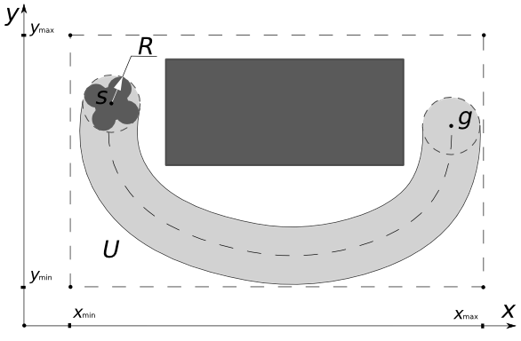
\includegraphics[width=0.9\textwidth]{pathtask.png}
				\begin{enumerate}
					\item Пусть $\pi(s,g)=(pos_1,pos_2,\dots,pos_m): los(pos_i,pos_{i+1})=true\ \forall i\in[1,m-1], pos_1=s,pos_m=g$.
					\item Траектория $tr(s,g)=[\pi(s,g),wait(m)]$, где $wait(s,g)=(wait_1,wait_2,\dots,wait_m)$ - множество временных задержек, $wait_1 \geq 0$.
					\item \underline{Задача}
					
					\textit{Дано}: $U,los,tr_1,\dots,tr_k,s,g$.
					
					\textit{Найти}: $tr(s,g)$ такую, что при движении вдоль этой траектории агент избегает столкновений со статическими и динамическими препятствиями.
					
					\textit{Критерий качества}: время следования по траектории.					
				\end{enumerate}
			\end{column}
		\end{columns}
	\end{frame}

	\begin{frame}
		\frametitle{Тактический уровень: графовая модель}
		\scriptsize
		\begin{columns}
			\begin{column}{0.6\textwidth}
				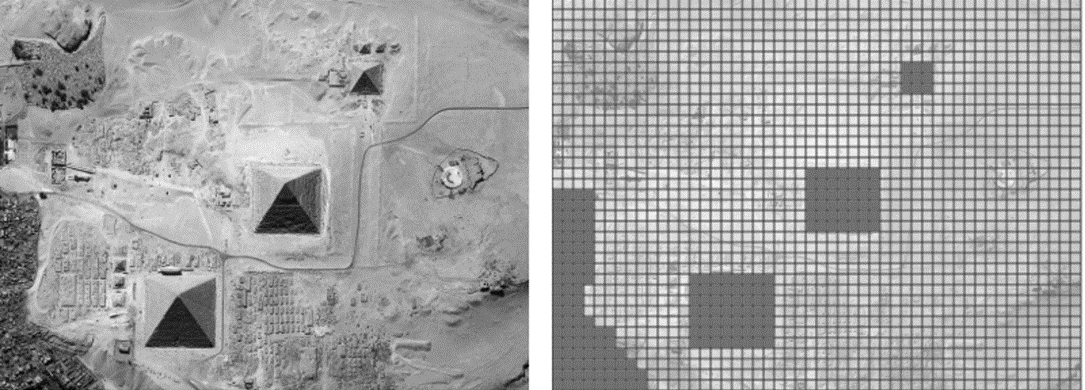
\includegraphics[width=0.9\textwidth]{grid.png}
				
				\textbf{Планирование как поиск пути на графе особого вида}
				\begin{itemize}
					\item Вершины $\rightarrow$ положения агента в пространстве.
					\item Ребра $\rightarrow$ элементарные траектории (отрезки).
					\item Веса ребер $\rightarrow$ длины соответствующих элементов траекторий.
					\item Путь на графе $\rightarrow$ траектория.
				\end{itemize}
				\par\medskip
				
				\textbf{Необходимо}
				\begin{itemize}
					\item Построить граф.
					\item Найти путь и рассчитать необходимые задержки при следовании по этому пути.
				\end{itemize}
			\end{column}
			\begin{column}{0.4\textwidth}
				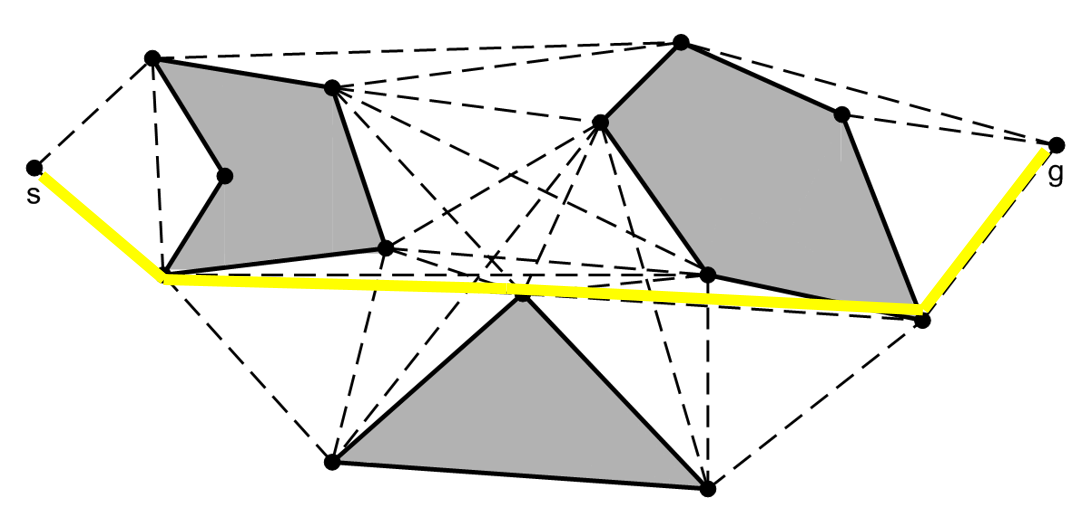
\includegraphics[width=0.9\textwidth]{pathobst.png}
				\begin{itemize}
					\item Агент(ы): открытый диск радиусом $r$.
					\item Размер клетки: $2r$.
					\item Положения агента(ов) - центры клеток.
				\end{itemize}
				\centering
				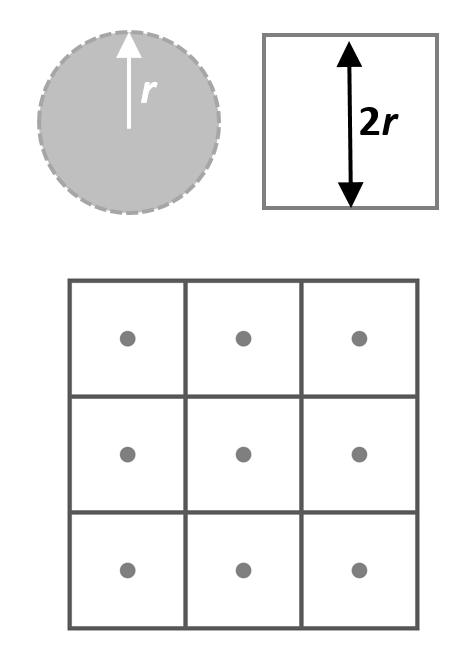
\includegraphics[width=0.4\textwidth]{pathdetails.png}
			\end{column}
		\end{columns}
	\end{frame}


	\begin{frame}
		\frametitle{Тактический уровень: алгоритм SIPP+Wait}
		\scriptsize
		\begin{columns}
			\begin{column}{0.6\textwidth}
				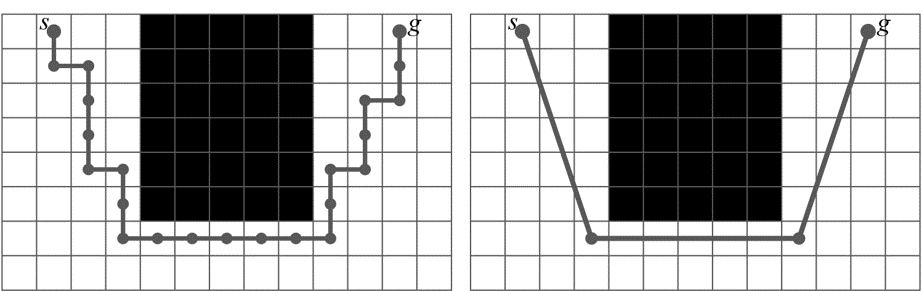
\includegraphics[width=\textwidth]{sipp.png}
			\end{column}
			\begin{column}{0.4\textwidth}
				\textbf{Традиционный подход}:
				
				Агент может перемещаться только в 4 (или 8) смежные вершины.
				\par\medskip
				\textbf{Рассматриваемый подход}:
				
				Агент может двигаться вдоль отрезка, который соединяет центры любых двух вершин (не обязательно смежных).
				
			\end{column}
		\end{columns}
		\par\medskip
		\small
		\textit{Идея}:
		\begin{itemize}
			\item Построить путь, т.е. пространственную компоненту траектории.
			\item Используя понятие безопасного интервала, определить необходимые задержки в каждой узловой точке.
		\end{itemize}
		
		
		\textit{Основное предполагаемое преимущество}
		
		\quad Высокая скорость работы
		
		\textit{Основной предполагаемый недостаток}

		\quad Недостаточное высокое качество решения
		
	\end{frame}

	\begin{frame}
		\frametitle{Тактический уровень: детали алгоритма}
		\footnotesize
		\begin{columns}
			\begin{column}{0.6\textwidth}
				\begin{itemize}
					\item Для проверки допустимости движения, необходимо найти все клетки, задеваемые агентом в процессе движения, и проверить их на проходимость.
					
					\item Если хотя бы одна из клеток непроходима - движение недопустимо.
					
					\item Конфликт между агентом и динамическим препятствием существует, если:
					\[
					|(pos + vt) - (pos' + v't)| = r_{rob} + r_{obs},
					\]
					т.е. существует момент времени, когда расстояние между агентом и динамическим препятствием меньше, чем сумма их радиусов.
					\item Определив существование конфликта, добавляем задержку и повторяем проверку.
				\end{itemize}
				
			\end{column}
			\begin{column}{0.4\textwidth}
				\centering
				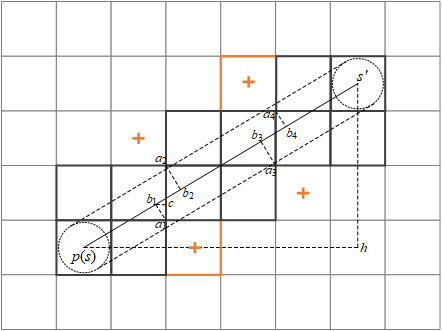
\includegraphics[width=\textwidth]{sippdetails.png}
				\par\bigskip
				Алгоритм Ву
				
				+
				
				\color{orange}Дополнительные проверки
				
				\color{black}=
				
				Алгоритм Ву+, который определяет все клетки, которые задевает агент.
				
			\end{column}
		\end{columns}
	\end{frame}


	\section{Стратегический уровень}
	
	\begin{frame}
		\frametitle{Картина мира субъекта деятельности}
		\scriptsize
			Картина мира субъекта деятельности - это представления субъекта о внешней среде, о своих собственных характеристиках, целях, мотивах, о других субъектах и операции (произвольные и непроизвольные), осуществляемые на основе этих представлений.
			\par\smallskip
			Элементом картины мира является знак:
			\begin{itemize}
				\item в смысле культурно-исторического подхода Выготского-Лурии,
				\item выполняющий функции в соответствии с теорией деятельности Леонтьева.
			\end{itemize}
			\begin{columns}
				\begin{column}{0.4\textwidth}
					\centering
					\includegraphics[width=0.6\textwidth]{signs/ru/sign_color_book_ru}
				\end{column}
				\begin{column}{0.6\textwidth}
					\begin{columns}
						\begin{column}{0.5\textwidth}
							\centering
							\includegraphics[width=\textwidth]{misc/phisio/ivan_cyrc}
						\end{column}
						\begin{column}{0.5\textwidth}
							\centering
							\includegraphics[width=\textwidth]{misc/phisio/workspace}
						\end{column}
					\end{columns}
					
				\end{column}
			\end{columns}
			В пользу существования такой структуры свидетельствуют:
			\begin{itemize}
				\item нейрофизиологические данные (Эдельман, Иваницкий, Маунткастл и др.),
				\item другие психологические теории (например, трехкомпонентная модель Станович).
			\end{itemize}
			\vspace{-5pt}
			\nocite{*}
			\printbibliography[keyword={sign}, resetnumbers=true]
	\end{frame}

	\begin{frame}
		\frametitle{Три образующих элемента картины мира}
		\scriptsize
		\begin{columns}
			\begin{column}{0.6\textwidth}
				\begin{center}
					\includegraphics[width=0.3\textwidth]{signs/ru/sign_colored}
				\end{center}
				\vspace{-5pt}
				Представляемая сущность описывается тремя причинно-следственными (каузальными) структурами:
				\begin{itemize}
					\item {\color{red}структура образа} - представление взаимосвязи внешних сигналов и внутренних характеристик субъекта (агента) - сенсо-моторное представление,
					\item {\color{blue}структура значения} - обобщенное знание о соотношениях во внешнем мире, согласованное в некоторой группе субъектов (агентов),
					\item {\color{green!60!black}структура личностного смысла} - ситуационная потребностно-мотивационная интерпретация знаний о соотношениях во внешней среде (значение для себя).
				\end{itemize}
			\end{column}
			\begin{column}{0.4\textwidth}
				\begin{center}
					\includegraphics[width=0.5\textwidth]{signs/en/sign_naming_colored_en}
				\end{center}
				\textbf{Процесс обучения} "--- образование новых знаков как неподвижной точки операторов замыкания 
				\[\Psi_p^m\Psi_m^a\Psi_a^p.\]
				\par\smallskip
				Реализация когнитивных функций "--- \textbf{актуализация} (активация) имеющихся знаков и формирование новых <<ситуационных>> знаков "--- <<протознаков>> без конвенционального имени.
			\end{column}
		\end{columns}
	\end{frame}

	\begin{frame}
		\frametitle{Каузальные матрицы и сети}
		\scriptsize
		\begin{center}
			\includegraphics[width=0.25\textwidth]{causnet/caus_matr}
			\quad\quad\quad
			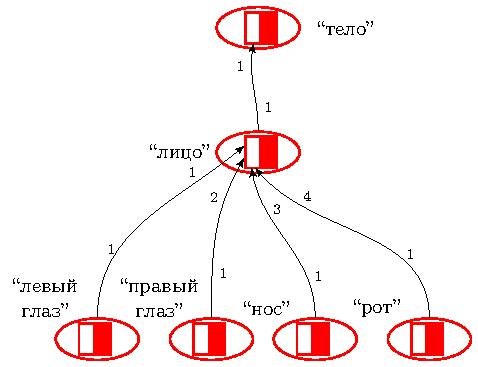
\includegraphics[page=1,width=0.25\textwidth]{examples/causnet/caus_net_colored}
		\end{center}
	
		\textbf{Каузальная сеть} на множестве образов знаков $W_p=\langle V_p, E_p \rangle$ - помеченный ориентированный граф, в котором
		\begin{itemize}
			\item каждому узлу $v\in V_p$ ставится в соответствие кортеж казуальных матриц $Z^p(s)$ образа некоторого знака $s$ ($v\rightarrow Z^p(s)$);
			\item ребро $e=(v_1, v_2)$ принадлежит множеству ребер графа $E$, если $v_1\rightarrow Z^p(s_1), v_2\rightarrow Z^p(s_2)$ и $s_1\in S_p(s_2)$;
			\item каждому ребру графа $e=(v_1, v_2), v_1\rightarrow Z^p(s_1), v_2\rightarrow Z^p(s_2)$ ставится в соответствие метка $\epsilon=(\epsilon_1,\epsilon_2,\epsilon_3)$ - кортеж трех натуральных чисел: $\epsilon_1$ - индекс исходной матрицы в кортеже $Z^p(s_1)$, может принимать специальное значение 0, если исходными могут служить любые матрицы из кортежа; $\epsilon_2$ - индекс целевой матрицы в кортеже $Z^p(s_2)$, строка которой ставится в соответствие признаку $s_1$; $\epsilon_2$ - индекс столбца в целевой матрице, в которой в соответствующей признаку $s_1$ строке стоит 1, может принимать положительные значения (\textit{столбцы условий}) и отрицательные (\textit{столбцы эффектов}).

		\end{itemize}
	\end{frame}
	
	\begin{frame}
		\frametitle{Планирование поведения}
		
		\begin{columns}
			\begin{column}{0.6\textwidth}
				\includegraphics[width=\textwidth]{algo/ru/beh_plan2_ru}
				\vspace{10pt}
				\nocite{*}
				\printbibliography[keyword={plan}, resetnumbers=true]
				\printbibliography[keyword={causnet}]
			\end{column}
			\begin{column}{0.4\textwidth}
				\scriptsize
				Иерархический процесс планирования начинается с конченой ситуации и стремится достичь начальной ситуации.
				\par\bigskip
				MAP-итерация:
				\begin{itemize}
					\item \textit{S-step} -- поиск прецедентов выполнения действия в текущих условиях,
					\item \textit{M-step} -- поиск применимых действий на сети значений,
					\item \textit{A-step} -- генерация личностных смыслов, соответствующих найденным значениям,
					\item \textit{P-step} -- построение новой текущей ситуации по множеству признаков условий найденных действий.
					
				\end{itemize}
			\end{column}
		\end{columns}
	\end{frame}
	
	\begin{frame}
		\frametitle{Представление пространственных знаний}
		\scriptsize
		\begin{columns}
			\begin{column}{0.5\textwidth}
				\centering
				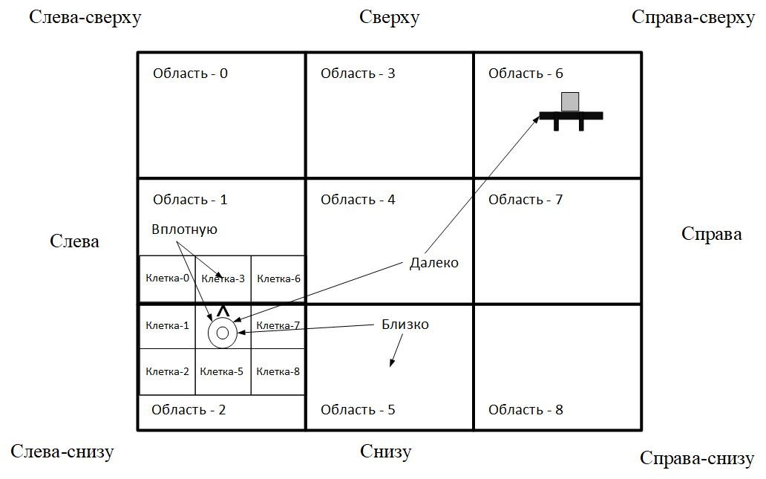
\includegraphics[width=0.85\textwidth]{behplan.png}
				
				\includegraphics[width=0.7\textwidth]{examples/representations/bica_psy_path.png}
			\end{column}
			\begin{column}{0.5\textwidth}
				\begin{itemize}
					\item Пространственная ситуация планирования описывается с использованием знакового представления (знаки областей, фокуса внимания, расстояний и направлений).
					\item Для задания пространственных отношений используется псевдофизическая пространственная логика Поспелова.
					\item Шаги планирования могут быть дополнены этапами рассуждений для пополнения текущей ситуации планирования.
					\item Элеменатрными операциями при выполнении плана являются функции планирования траектории.
				\end{itemize}
			\end{column}
		\end{columns}
	
		\nocite{*}
		\printbibliography[keyword={behplanrus}, resetnumbers=true]
	\end{frame}

	\begin{frame}
		\frametitle{Знаки Я и Они в алгоритме планирования MAP}
		
		\begin{center}
			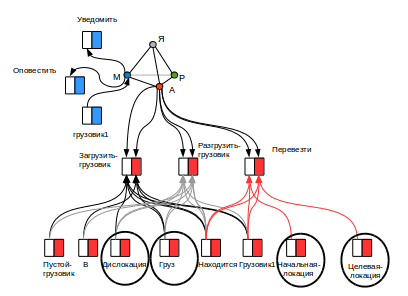
\includegraphics[width=0.45\textwidth]{I-sign.png}
			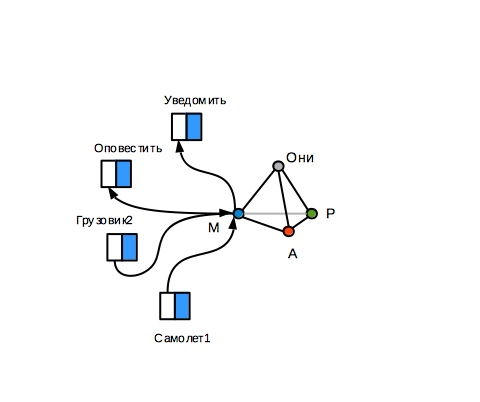
\includegraphics[width=0.45\textwidth]{they-sign.png}
		\end{center}
		\nocite{*}
		\printbibliography[keyword={roledistrib}, resetnumbers=true]
	\end{frame}

	\begin{frame}
		\frametitle{Реализация на реальных роботах и моделях}
		
		\begin{center}
			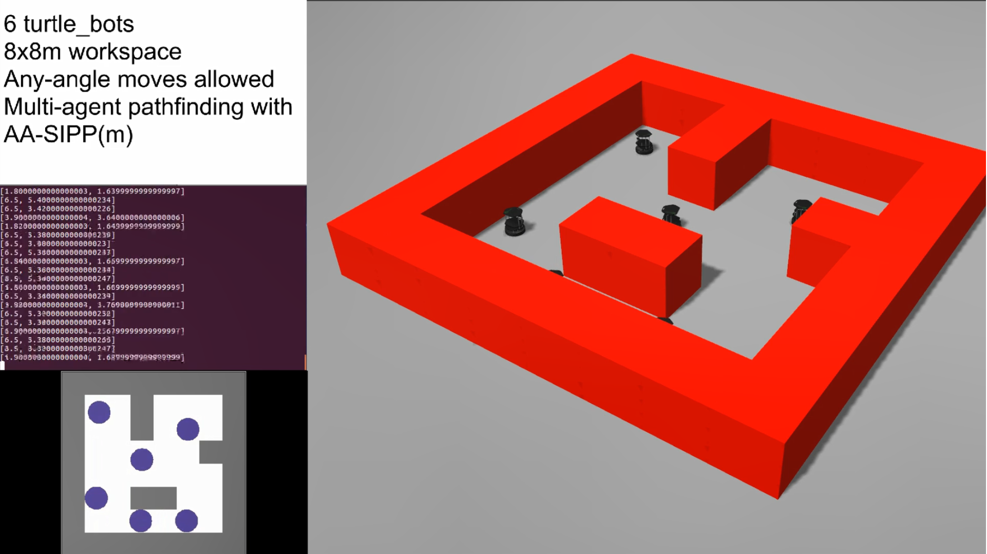
\includegraphics[width=0.6\textwidth]{gazebo.png}
			\quad\quad
			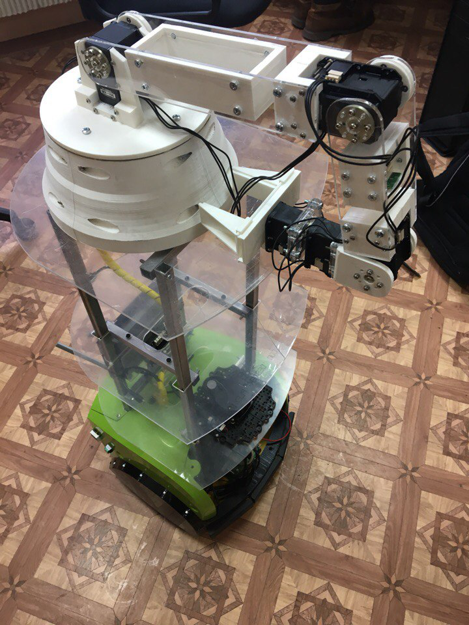
\includegraphics[width=0.3\textwidth]{nexus.png}
		\end{center}
	\end{frame}
	
	\section{Заключение}

	\begin{frame}
		\frametitle{Список публикаций}
		
		\nocite{*}
		\printbibliography[keyword={fulllist}, resetnumbers=true]
		\end{frame}	
		
		\begin{frame}
		\frametitle{Направления исследований и будущие работы}
		\scriptsize
		\begin{itemize}
		\item Реализация элементов логического вывода в знаковой картине мира.
		\item Развитие кортикоморфных алгоритмов обучения.
		\item Разработка иерархических методов обучения с подкреплением и интеграция их в алгоритмы семейства MAP.
		\item Моделирование рефлексивного поведния, например, добавление этапа выбора эвристики при планирования поведения (reflectiveMAP).
		\item Интеграция этапа выполнения в общий цикл планирования и уточнение этапа перепланирования.
		\item Подробная разработка алгоритмов коммуникации и согласования знаний.
		\end{itemize}
		\par\bigskip
		\tikz[baseline]{
		\node[fill=blue!20, rounded corners=5pt, minimum width=330, minimum height = 75] (k2) {
		\begin{minipage}[t][75pt]{330pt}
			\normalsize
			Приглашаем студентов и аспирантов для участия в научной работе по направлениям работы отдела:
			\begin{itemize}
				\item курсовая и проектная работа в базовой кафедре МФТИ,
				\item аспирантура в ФИЦ ИУ РАН,
				\item стажировки (в т.ч. и оплачиваемые) в SLabAI.
			\end{itemize}
		\end{minipage}
		
		};
		}
	
	\end{frame}
	
	\begin{frame}
		\frametitle{Анонсы}
		\small
		\begin{itemize}
			\item XVI Национальная конференция по искусственному интеллекту (КИИ 2018) "--- крупнейшее академическое мероприятие в области ИИ в России (24-27 сентября, подача - 14 апреля).
			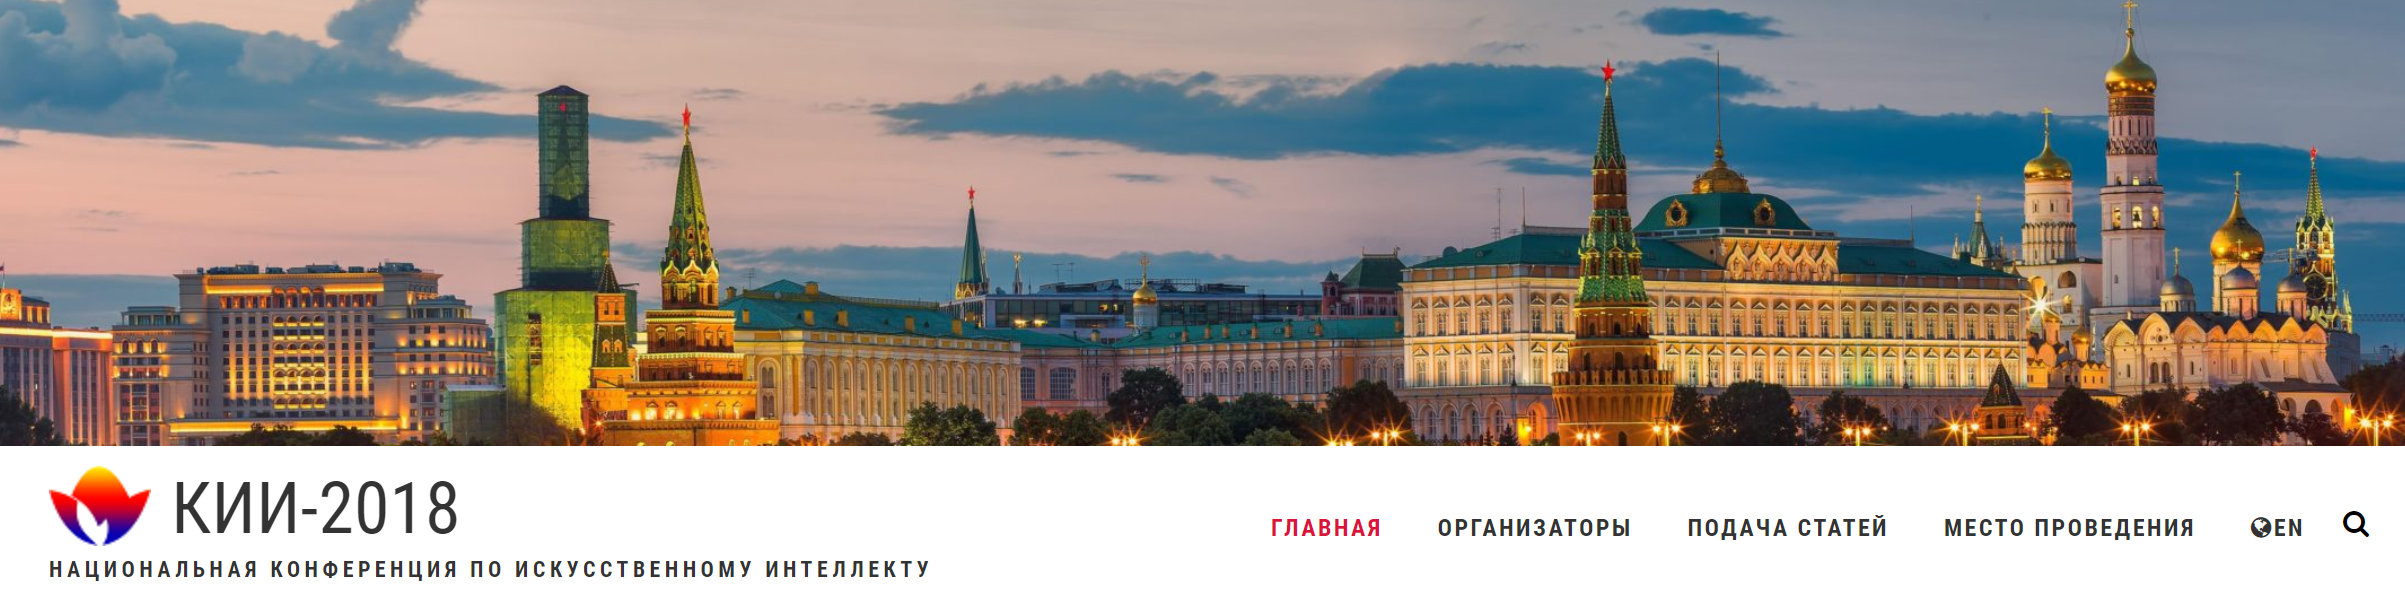
\includegraphics[width=0.8\textwidth]{rncai.png}
			\item Пятая всероссийская научная конференция молодых ученых с международным участием <<Информатика, Управление и Системный Анализ>> (ИУСА-2018) (6-8 июня).
			
\includegraphics[width=0.8\textwidth]{icsa.png}
		\end{itemize}
	\end{frame}
	
	\begin{frame}
		\centering
		\Huge
		Спасибо за внимание!
		\normalsize
		\par\bigskip
		Дополнительно лекции на Постнауке (\url{https://postnauka.ru/author/panov}):
		\par\medskip
		{\footnotesize
		Когнитивная робототехника "--- \url{https://postnauka.ru/video/77709}
		
		Компьютерное когнитивное моделирование "--- \url{https://postnauka.ru/video/79133}
		
		Идеи нейрофизиологии в ИИ "--- \url{https://postnauka.ru/video/81699}
		}
		\par\bigskip
		pan@isa.ru
		\par\bigskip
		Репозиторий "--- \url{https://github.com/cog-isa}
		
		Канал Youtube "--- \url{https://www.youtube.com/channel/UChkz6VVLv9KJJg9XTcR0CLQ}
	\end{frame}	
\end{document}
	
	
